\chapter{Meshes in \fluidity}\label{chap:meshes}
\index{mesh!generation}
\index{grid|see{mesh}}

In each run of \fluidity\ an input mesh needs to 
be provided. Even in adaptive mesh runs an initial mesh is needed
to define the initial condition of the fields on. 
This chapter covers a number of topics 
related to meshes in \fluidity:  what
mesh formats are supported (section \ref{sec:supported_mesh_formats})
, how different regions and boundary surfaces can be
marked (section \ref{sec:surface_and_region_ids}), 
the relation between meshes and function spaces (section
\ref{sec:meshes_and_function_spaces}), the extrusion of 
horizontal meshes in the vertical (section \ref{sec:extruded_meshes}), 
the creation of periodic meshes (section \ref{sec:periodic_meshes}),
and finally an overview of meshing tools provided with \fluidity (section
\ref{sec:meshing_tools}).

\section{Supported mesh formats}
\label{sec:supported_mesh_formats}
\fluidity\ supports two mesh file formats:
\begin{enumerate}
\item Gmsh .msh files. Gmsh is a mesh generator freely available on the
web at \url{http://geuz.org/gmsh/}, and is included in Linux distributions 
such as Ubuntu. This is the recommended file format.
\item Triangle format. This is stored as a set of 3 files: a .node file,
a .ele file and a .face (3D) or .edge (2D) or .bound (1D) file. This file format
is mainly supported for special purposes, like 1D meshes, and some offline 
tools.
\end{enumerate}

For a detailed, technical description of the two mesh file formats see 
appendix~\ref{chap:mesh_formats}. In addition, instructions on how
to generate a mesh using Gmsh in simple geometries as well as complex
ocean domains can be found in the Gmsh tutorial available at
\url{http://amcg.ese.ic.ac.uk/files/amcg-gmsh-tutorial.pdf}

\section{Surface and regions ids}
\label{sec:surface_and_region_ids}
\index{surface ID}
\index{region ID}
Surface ids are used in \fluidity\ to mark different parts of the boundary of the
computational domain so that different boundary conditions can be associated
with them. Regions ids are used to mark different parts of the domain itself.
Both ids can be defined in Gmsh by assigning physical ids to different
geometrical objects. In two dimensions surface ids can be defined by assigning a
physical id to each group of lines that make up a part of the boundary that
needs to be considered separately. Region ids can be defined by dividing the
domain up in different (groups of) surfaces and assigning different 
physical ids to them. Similarly, in three dimensions surface ids are defined by
assigning physical surface ids in Gmsh, and regions ids by assigning physical
volume ids.

It is recommended, and required in parallel, that all parts of the domain
boundary are marked with a surface id. Region ids are optional. They can be used
to instruct the adaptivity library to strictly maintain the interface between 
different regions of the domain. They are also useful to set different constant 
field values in the regions.

\section{Meshes and function spaces}
\label{sec:meshes_and_function_spaces}
\index{mesh!coordinate mesh}
\index{mesh!nodes}
\index{mesh!simplicial}
\index{mesh!cubical}
The choice of computational mesh directly controls how the fields (velocity,
pressure, temperature, etc.) of the model are discretised. For example, using a
triangular mesh with a \Pone continuous Galerkin discretisation, the field
values are stored in the vertices of the mesh and the field is linearly
interpolated inside the triangles. For a discontinuous \PoDG discretisation the
field values are stored in the three corners of each triangle separately. The
locations of these field values are referred to as nodes. As another example, the
nodes of the \Ptwo discretisation correspond to the triangle vertices, and the
midpoints of the edges.

This combination of the set of polygons (triangles, tetrahedrals, 
quadrilaterals, etc.) covering the domain 
and a choice of polynomial order and continuity between
elements (\Pone, \PoDG, \Ptwo, etc.) therefore defines the discrete function 
space in which the approximate discrete fields are found, and the nodes
in which the field values are stored. In \fluidity\ 
the term mesh is often used to refer to this specific combination, and fields are said
to be defined on such meshes. In other words ``meshes'' in \fluidity\ correspond
to the (polynomial) discrete function spaces.

Both simplicial meshes (triangles in 2D and tetrahedrals in 3D) and cubical
meshes (quadrilaterals in 2D and hexagons in 3D) are supported. Note however
that the choice between these two types of input meshes also has an influence
on the function space. For simplicial meshes, a polynomial order
of one means linear polynomials are used (\Pone), whereas in cubical meshes this
leads to bilinear (trilinear in 3D) polynomials (known as the \Qone
discretisation). Therefore to use 
the \Poo or the \PoDGPt discretisation 
a simplicial input mesh is needed. Structured meshes in two
or three dimensions can be generated by stacking two triangles in a rectangle,
or six tetrahedrals in a cube respectively. Such meshes are easily obtained
using Gmsh.

In mixed finite element discretisations, where different fields are discretised
using different function spaces (again \PoDGPt is a clear example), a mesh needs
to be defined for every function space that is used. In \fluidity, 
the input mesh is always considered to be a 
continuous linear mesh (\Pone for simplicial and \Qone for
cubical meshes), as its vertices correspond to the nodes of the \Pone/\Qone
discretisation. For a \PoDGPt discretisation we therefore need two additional
meshes: a \PoDG mesh and \Ptwo mesh. In section \ref{sec:mesh_configuration} it
is explained how these can be derived from the input mesh.

In finite element discretisations the actual shape of the elements in physical
space is given by a function from local coordinates on the element to
coordinates in physical space, the coordinate map. This map is typically linear,
resulting in elements with straight edges. For some applications, for example
ocean models on the sphere, it may be desirable to use higher order
polynomials however, so that large elements can be bended to fit the
geometry. The mesh (function space) that is used for the coordinate map is
referred to as the coordinate mesh. For standard, uncurved elements 
the coordinate mesh simply corresponds to the (linear) input mesh
(except for periodic meshes, see section \ref{sec:periodic_meshes} below).

\section{Extruded meshes}
\label{sec:extruded_meshes}
\index{mesh!extruded}

Given a 1D or 2D input mesh, \fluidity\ can extrude this
mesh to create a layered 2D or 3D mesh, on which simulations can be
performed. The extrusion is always downwards (in the direction of gravity), 
and the top of the domain is always flat, corresponding to the $y=0$-level 
in 2 dimension, the $z=0$ level in 3 dimensions, or the equilibrium 
free surface geoid when running on the sphere.

The advantage of this approach is that the user can provide a horizontal mesh,
that has been created in the normal way (usually Gmsh), and all the
configuration related to bathymetry, number of layers and layer depths can be
done in the .flml (see section \ref{sec:extruded} for all options available). It also
enables the application of mesh adaptivity in the horizontal and vertical
independently. This means we can choose to apply adaptivity in the horizontal
only and keep a fixed number of layers, or we can choose to keep the horizontal
mesh fixed and dynamically adjust the vertical grid spacing (vertical
adaptivity). The combination of both horizontal and vertical adaptivity is
referred to as ``2+1D'' adaptivity. For the configuration of this kind of
adaptivity see section \ref{sec:vertically_structured_adaptivity}.

\section{Periodic meshes}
\index{mesh!periodic} 
\index{periodic domain} 
\label{sec:periodic_meshes}
Periodic meshes are those that are ``virtually'' connected on one side of the
domain to the boundary on the opposite side. This can be done in one or more
directions. To make a periodic
mesh you must first create an input mesh where the edges on the two sides
that will be connected
can be mapped exactly by a simple transformation. For a 2d mesh that is 
periodic in the $x$-direction this simply means all the nodes on left and right
boundary need to be at the same $y$-height. For 3d meshes, not only the nodes
on the two sides need to be ``periodic'', but also the edges connecting them.
For a simple box geometry, this can be easily accomplished using the
\lstinline[language=Bash]+create_aligned_mesh+ script in the tools folder.

Alternatively, if you require a more complex periodic mesh with some structure between the periodic 
boundaries you can create one using \lstinline[language=Bash]{gmsh}. This can be achieved by 
setting up the periodic boundaries by using extrude and then deleting the 'internal' mesh.

The use of periodic domains requires additional configuration options. See
section \ref{sec:periodic}.

\section{Meshing tools}
\label{sec:meshing_tools}
\index{mesh!meshing tools}

There are a number of meshing tools in tools directory. These can be built by running 
\lstinline[language = bash]+make fltools+ in the top directory of the \fluidity\ trunk.
The following binaries will then be created in the \lstinline+bin/+ directory (see section \ref{sec:fltools}).

\subsection{Mesh Verification}
\index{mesh!meshing tools!mesh verification}

The \lstinline[language = Bash]+checkmesh+ tool can be used to form a number of verification tests on a mesh
in triangle mesh format. More information can be found in section~\ref{sec:checkmesh}.

\subsection{Mesh creation}
\index{mesh!meshing tools!mesh creation}
The \lstinline[language = bash]+interval+ tool (section~\ref{sec:interval}) generates a 1D line mesh in triangle format. 

The \lstinline[language = bash]+gen_square_meshes+ tool (section~\ref{sec:gen_square_meshes})  will generate triangle files for multiple 2D square meshes with a specified number of internal nodes.

The \lstinline[language = bash]+create_aligned_mesh+ tool (section~\ref{sec:create_aligned_mesh}) creates the triangle files for a mesh that lines up in all directions, so that it can be made it into a singly, doubly or triply periodic mesh.

\subsection{Mesh conversion}
\index{mesh!meshing tools!mesh conversion}

The \lstinline[language = Bash]+gmsh2triangle+ tool (section~\ref{sec:gmsh2triangle}) converts ASCII Gmsh mesh files into triangle format.

The \lstinline[language = Bash]+triangle2vtu+ tool (section~\ref{sec:triangle2vtu}) can be used to convert triangle format files into vtu format. 

The \lstinline[language = Bash]+gmsh_mesh_transform+ script (section~\ref{sec:gmsh_mesh_transform}) applies a coordinate transformation to a region of a given mesh. 

\subsection{Decomposing meshes for parallel}
\label{decomp_meshes_parallel}
\index{parallel!mesh decomposition}
To run in parallel one must first divide the mesh into a number of blocks, a process
commonly referred to as \emph{mesh decomposition}. Figure \ref{fig:NACA0025_mesh_with_partitions}
shows a possible partition of an example mesh. When \fluidity\ is run in parallel (see section
\ref{sec:running_fluidity_in_parallel}), each processor then reads the mesh corresponding to a
single block. This section outlines how to decompose a mesh with \fluidity\ tools.
\begin{figure}[htbp]
 \centering
  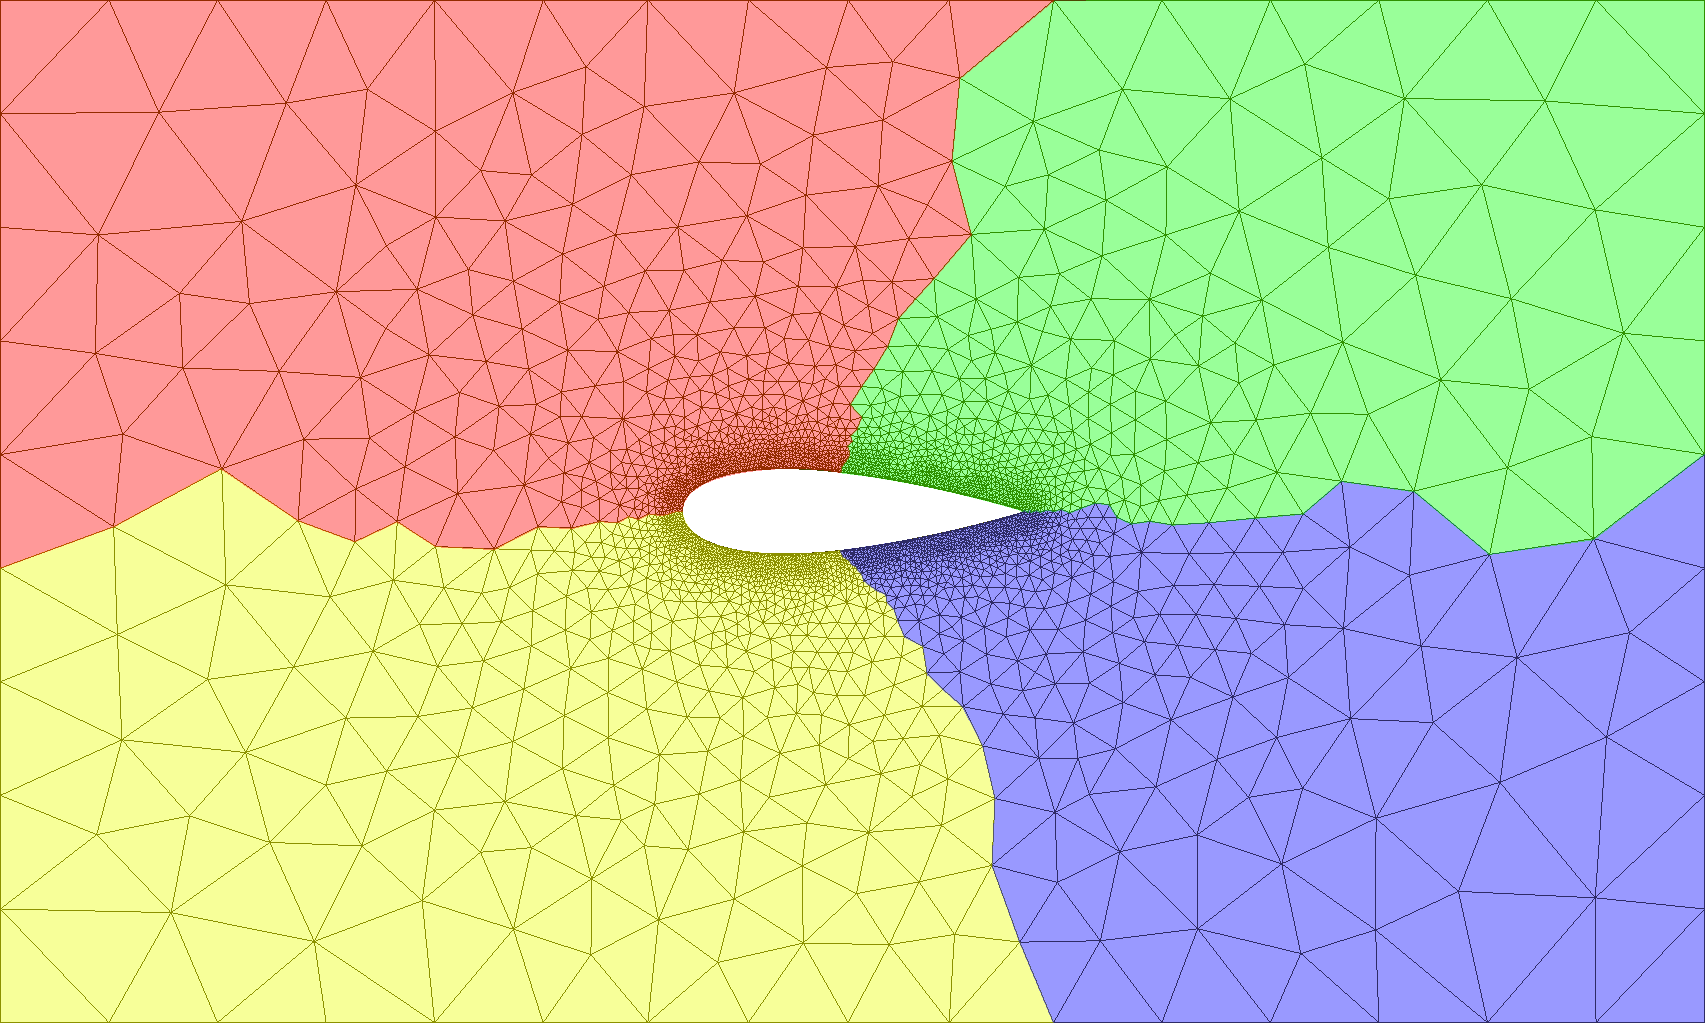
\includegraphics[width=0.7\textwidth]{misc_images/NACA0025_mesh_with_partitions.pdf}
  \caption{An unstructured mesh around a NACA0025 aerofoil, the coloured patches show a
           possible decomposition into 4 partitions.}
  \label{fig:NACA0025_mesh_with_partitions}
\end{figure}

\subsubsection{fldecomp}
\index{mesh!meshing tools!fldecomp}
\label{mesh!meshing tools!fldecomp}

\lstinline[language=bash]+fldecomp+ can be used to decompose a mesh. For example, if your mesh
file is \lstinline[language=bash]+foo.msh+ and you want to decompose into four parts, type:
\begin{lstlisting}[language = Bash]
`\fluiditysourcepath'/bin/fldecomp -n 4 -m gmsh foo
\end{lstlisting}
See section \ref{sec:fldecomp} for more details.

\subsubsection{flredecomp}
\index{mesh!meshing tools!flredecomp}
\label{mesh!meshing tools!flredecomp}
\lstinline[language=bash]+flredecomp+ is a tool similar to \lstinline[language=bash]+fldecomp+ but runs in parallel. 
It performs a re-decomposition of a Fluidity checkpoint.
For example, to decompose the serial file \lstinline+foo.flml+
into four parts, running on 4 processors type:

\begin{lstlisting}[language=bash]
mpiexec -n 4 `\fluiditysourcepath'/bin/flredecomp \
    -i 1 -o 4 foo foo_flredecomp
\end{lstlisting}

The output of running flredecomp is a series of mesh and vtu files as well
as the new flml; in this case \lstinline+foo_flredecomp.flml+. 
Note that \lstinline[language=bash]+flredecomp+ must be run on a number of processors equal to the larger number of processors between input and output.

When using flredecomp, it is possible to partition the mesh based upon a user defined weighting. 
This is achieved by prescribing a scalar field, bounded between values of 0 and 1, under 
\option{/flredecomp/field\_weighted\_partitions}. Flredecomp will then try to ensure that the sum 
of weights on each partition is approximately equal.

Further information on flredecomp can be found in section~\ref{sec:flredecomp}.

\subsection{Decomposing a periodic mesh}
\index{mesh!meshing tools!periodise}
\label{sec:decomposing_meshes_periodise}

To be able to run \fluidity\ on a periodic mesh in parallel you have to use
two tools:

\begin{itemize}
\item periodise (section \ref{sec:periodise})
\item flredecomp (section \ref{sec:flredecomp})
\end{itemize}

The input to \lstinline+periodise+ is your flml (in this case
\lstinline{foo.flml}). This flml file should already contain the mapping for
the periodic boundary as described in section
\ref{sec:periodic}. Periodise is run with the command:

\begin{lstlisting}[language=bash]
`\fluiditysourcepath'/bin/periodise foo.flml
\end{lstlisting}

The output is a new flml called \lstinline+foo_periodised.flml+ and the
periodic meshes. Next run flredecomp (section \ref{sec:flredecomp}) to decompose the mesh for the number of processors
required. The flml output by flredecomp is then used to execute the actual simulation:

\begin{lstlisting}[language=bash]
mpiexec -n [number of processors] \
   `\fluiditysourcepath'/bin/fluidity [options] \
   foo_periodised_flredecomp.flml
\end{lstlisting}

\section{Non-\fluidity\ tools}

In addition to the tools and capabilities of \fluidity, there are numerous
tools and software packages available for mesh generation. Here, we describe 
two of the tools commonly used.

\subsection{Terreno}
\index{mesh!meshing tools!Terreno}
\index{Terreno}

Terreno uses a 2D anisotropic mesh optimisation algorithm to explicitly optimise for 
element quality and bathymetric approximation while minimising the number of mesh
elements created. The shoreline used in the mesh generation process is the result 
of a polyline approximation algorithm that where the minimum length of the resulting 
edges is considered as well as the distance an edge is from a vertex on the original 
shoreline segment being approximated. The underlying philosophy is that meshing and 
approximation should be error driven and should minimise user intervention. The 
latter point is two pronged: usability is paramount and the user should not need 
to be an expert in mesh generation to generate high quality meshes for their ocean 
model; fundamentally there must be clearly defined objectives to the mesh generation 
process to ensure reproducibility of results. The result is an unstructured mesh, 
which may be anisotropic, which focuses resolution where it is required to optimally 
approximate the bathymetry of the domain. The criterion to judge the quality of the 
mesh is defined in terms of clearly defined objectives. An important feature of the 
approach is that it facilitates multi-objective mesh optimisation. This allows one to 
simultaneously optimise the approximation to other variables in addition to the 
bathymetry on the same mesh, such as back-scatter data from soundings, material 
properties or climatology data. 

See the \href{http://amcg.ese.ic.ac.uk/terreno}{Terreno website}\ for more information.

\subsection{Gmsh}
\index{mesh!meshing tools!gmsh}
\index{gmsh}
\label{sec:meshing_tools_non_fluidity_gmsh}

Gmsh is a 3D finite element mesh generator with a build-in CAD engine and post-processor.
Its design goal is to provide a fast, light and user-friendly meshing tool with parametric
input and advanced visualisation capabilities. Gmsh is built around four modules: geometry, 
mesh, solver and post-processing. The specification of any input to these modules is done
either interactively using the graphical user interface or in ASCII text files using Gmsh's
own scripting language. 

For more information see the \href{http://geuz.org/gmsh/}{Gmsh website}\ or the \href{http://amcg.ese.ic.ac.uk}{AMCG
website}. An online manual is available at \href{http://geuz.org/gmsh/doc/texinfo/gmsh.html}{geuz.org/gmsh/doc/texinfo/gmsh.html}.

\subsection{Importing contours from bathymetric data into Gmsh}
\index{mesh!generation!gmsh!entering! bathymetry! data! into! fluidity! using! Gmsh}
\index{Entering bathymetry data into fluidity using Gmsh}

Gmsh can be used to create a mesh of a `real' ocean domain for use with \fluidity. An online guide to using Gmsh's built in
GSHHS plug-in is available at \href{http://perso.uclouvain.be/jonathan.lambrechts/gmsh_ocean/}{gmsh\_ocean}.
It is also possible to import contours from arbitrary bathymetry data sources into Gmsh. A guide and sample code detailing this process will
in the future be available on the \href{http://amcg.ese.ic.ac.uk}{AMCG website}.
